Let $\vec{O}$ be the centre and $r$ be the radius of the given circle.
\\
$\therefore$
\begin{align}
    \label{eq:quad_form/2/1}
    \begin{split}
\vec{O} &= \myvec{p\\0}
\\
r &= 5
    \end{split}
\end{align}

The general equation of a circle is given by 
\begin{align}
\vec{x}^T\vec{x} - 2\vec{O}^T\vec{x} + \norm{\vec{O}}^2 -r^2 = 0
\end{align}
which, upon substitution from \eqref{eq:quad_form/2/1} yields
\begin{align}
\vec{x}^T\vec{x} - 2\myvec{p & 0}\vec{x} + p^2 - 25 = 0
\end{align}
$\because$
Point $\vec{A}$=\myvec{2\\3} lies on the circle, 
%
\begin{align}
\myvec{2 & 3}\myvec{2\\3} - 2\myvec{p & 0}\myvec{2\\3} + p^2 -25 &=0
\\
\implies p^2 - 4p - 12 &=0
\\
\implies p &=6 
\text{ or } -2
\end{align}

Hence,the possible equations of the circle are
\begin{align}
\vec{x}^T\vec{x} - 2\myvec{6 & 0}\vec{x} + 11 &= 0 \label{quad_form/2/1eq:1}
\\
\text{or}, \vec{x}^T\vec{x} - 2\myvec{-2 & 0}\vec{x} - 21 &= 0 \label{quad_form/2/1eq:2}
\end{align}

which are plotted in Fig. \ref{quad_form/2/1fig:circle}	


\begin{figure}[!ht]
\centering
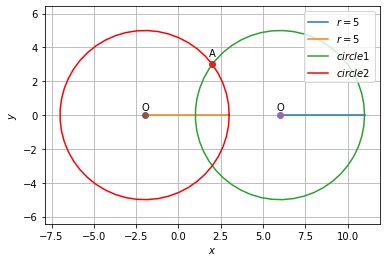
\includegraphics[width=\columnwidth]{solutions/su2021/2/1/Figure5.png}
\caption{Circles with centres (6,0) and (-2,0) respectively }
\label{quad_form/2/1fig:circle}	
\end{figure}


